\documentclass[a4paper,10pt,dvipdfmx]{jsarticle}
\usepackage{graphicx}
\usepackage{amsmath,amssymb,amsthm,bm}
\usepackage{booktabs,multirow,array}
\usepackage{xcolor}
\usepackage[top=19mm,bottom=21mm,left=19mm,right=19mm]{geometry}
\newtheorem{theorem}{定理}
\newtheorem{proposition}{命題}
\newtheorem{corollary}{系}
\theoremstyle{definition}
\newtheorem{definition}{定義}
\renewcommand{\proofname}{証明}
\newcommand{\cS}{\mathcal{S}}
\newcommand{\cR}{\mathcal{R}}
\newcommand{\cC}{\mathcal{C}}
\newcommand{\cT}{\mathcal{T}}
\newcommand{\cU}{\mathcal{U}}
\newcommand{\hQ}{\hat{Q}}
\newcommand{\E}{\mathbb{E}}
\newcommand{\AUC}{AUROC}
\newcommand{\FPR}{FPR95}
\newcommand{\pP}{p^{+}}
\newcommand{\pN}{p^{-}}
\newcommand{\pfin}{p^{\mathrm{fin}}}
\newcommand{\tabref}[1]{表\ref{#1}}
\newcommand{\figref}[1]{図\ref{#1}}
\newcommand{\NAbsOneFar}{28.27}
\newcommand{\NAbsOneFarAuc}{90.74}
\newcommand{\NAbsOneFarTpr}{71.2}
\newcommand{\NAbsOneFarVal}{0.047}
\newcommand{\NAbsOneFarValTwo}{0.196}
\newcommand{\NAbsOneGapFar}{11.53}
\newcommand{\NAbsOneGapNear}{-0.26}
\newcommand{\NAbsOneHiFar}{27.29}
\newcommand{\NAbsOneHiFarAuc}{91.24}
\newcommand{\NAbsOneHiFarTpr}{72.3}
\newcommand{\NAbsOneHiFarVal}{0.048}
\newcommand{\NAbsOneHiFarValTwo}{0.197}
\newcommand{\NAbsOneHiNear}{13.73}
\newcommand{\NAbsOneHiNearAuc}{96.33}
\newcommand{\NAbsOneHiNearTpr}{86.8}
\newcommand{\NAbsOneHiNearVal}{0.053}
\newcommand{\NAbsOneHiNearValTwo}{0.199}
\newcommand{\NAbsOneMinusSigFar}{+11.53}
\newcommand{\NAbsOneMinusSigNear}{-0.26}
\newcommand{\NAbsOneNear}{13.43}
\newcommand{\NAbsOneNearAuc}{96.02}
\newcommand{\NAbsOneNearTpr}{86.8}
\newcommand{\NAbsOneNearVal}{0.052}
\newcommand{\NAbsOneNearValTwo}{0.201}
\newcommand{\NAbsPoolFar}{25.35}
\newcommand{\NAbsPoolFarAuc}{91.65}
\newcommand{\NAbsPoolFarIdf}{18.6}
\newcommand{\NAbsPoolFarSeeds}{1,164}
\newcommand{\NAbsPoolFarTpr}{74.3}
\newcommand{\NAbsPoolFarVal}{0.049}
\newcommand{\NAbsPoolFarValTwo}{0.199}
\newcommand{\NAbsPoolNear}{14.19}
\newcommand{\NAbsPoolNearAuc}{96.53}
\newcommand{\NAbsPoolNearIdf}{19.8}
\newcommand{\NAbsPoolNearSeeds}{5,359}
\newcommand{\NAbsPoolNearTpr}{86.0}
\newcommand{\NAbsPoolNearVal}{0.051}
\newcommand{\NAbsPoolNearValTwo}{0.198}
\newcommand{\NAbsXfitFar}{24.40}
\newcommand{\NAbsXfitFarAuc}{92.01}
\newcommand{\NAbsXfitFarIdf}{18.9}
\newcommand{\NAbsXfitFarSeeds}{1,291}
\newcommand{\NAbsXfitFarTpr}{75.3}
\newcommand{\NAbsXfitFarVal}{0.049}
\newcommand{\NAbsXfitFarValTwo}{0.198}
\newcommand{\NAbsXfitNear}{13.81}
\newcommand{\NAbsXfitNearAuc}{96.63}
\newcommand{\NAbsXfitNearIdf}{20.2}
\newcommand{\NAbsXfitNearSeeds}{5,515}
\newcommand{\NAbsXfitNearTpr}{86.3}
\newcommand{\NAbsXfitNearVal}{0.051}
\newcommand{\NAbsXfitNearValTwo}{0.198}
\newcommand{\NCkAdd}{2e-15}
\newcommand{\NCkExit}{6e-17}
\newcommand{\NCkFates}{2e-15}
\newcommand{\NCkKcl}{2e-14}
\newcommand{\NCkLgcSpHi}{0.9998}
\newcommand{\NCkLgcSpLo}{0.55}
\newcommand{\NCkLgcSpreadHi}{3e-02}
\newcommand{\NCkLimFour}{0.031}
\newcommand{\NCkLimTwo}{0.77}
\newcommand{\NCkMcMaxZ}{0.9}
\newcommand{\NCkPhiMax}{0.49}
\newcommand{\NCkPhiMin}{0.14}
\newcommand{\NCkPiMax}{0.22}
\newcommand{\NCkPoolFdp}{0.155}
\newcommand{\NCkPoolFdpSe}{0.003}
\newcommand{\NCkPoolFive}{0.050}
\newcommand{\NCkPoolFiveSe}{0.001}
\newcommand{\NCkPoolTen}{0.101}
\newcommand{\NCkPoolTenSe}{0.001}
\newcommand{\NCkPoolTwenty}{0.201}
\newcommand{\NCkPoolTwentySe}{0.001}
\newcommand{\NCkQmm}{0.167}
\newcommand{\NCkReps}{400}
\newcommand{\NCkScale}{2e-15}
\newcommand{\NCkSepELeAct}{100}
\newcommand{\NCkSepELeBnd}{94}
\newcommand{\NCkSepEN}{160}
\newcommand{\NCkSepEPi}{0.045}
\newcommand{\NCkSepERhoOm}{0.27}
\newcommand{\NCkSepEViol}{0}
\newcommand{\NCkSepN}{154}
\newcommand{\NCkSepViol}{0}
\newcommand{\NCkTonlyFdp}{0.175}
\newcommand{\NCkTonlyFdpSe}{0.003}
\newcommand{\NCkTonlyFive}{0.054}
\newcommand{\NCkTonlyFiveSe}{0.001}
\newcommand{\NCkTonlyTen}{0.104}
\newcommand{\NCkTonlyTenSe}{0.001}
\newcommand{\NCkTonlyTwenty}{0.202}
\newcommand{\NCkTonlyTwentySe}{0.001}
\newcommand{\NCtHitFar}{15.29}
\newcommand{\NCtHitFarAuc}{96.72}
\newcommand{\NCtHitFarTpr}{84.4}
\newcommand{\NCtHitFarVal}{0.049}
\newcommand{\NCtHitFarValTwo}{0.201}
\newcommand{\NCtHitNear}{19.81}
\newcommand{\NCtHitNearAuc}{95.71}
\newcommand{\NCtHitNearTpr}{80.6}
\newcommand{\NCtHitNearVal}{0.052}
\newcommand{\NCtHitNearValTwo}{0.204}
\newcommand{\NDegAucFarD}{82.2}
\newcommand{\NDegAucFarL}{86.7}
\newcommand{\NDegAucNearD}{48.6}
\newcommand{\NDegAucNearL}{49.1}
\newcommand{\NDegFprFarD}{70.6}
\newcommand{\NDegFprFarL}{61.6}
\newcommand{\NDegFprNearD}{95.8}
\newcommand{\NDegFprNearL}{95.5}
\newcommand{\NDegSpFarD}{0.82}
\newcommand{\NDegSpFarL}{0.80}
\newcommand{\NDegSpNearD}{0.50}
\newcommand{\NDegSpNearL}{0.46}
\newcommand{\NDirFar}{38.92}
\newcommand{\NDirFarAuc}{87.87}
\newcommand{\NDirFarTpr}{60.3}
\newcommand{\NDirFarVal}{0.047}
\newcommand{\NDirFarValTwo}{0.195}
\newcommand{\NDirNear}{16.36}
\newcommand{\NDirNearAuc}{95.20}
\newcommand{\NDirNearTpr}{83.6}
\newcommand{\NDirNearVal}{0.050}
\newcommand{\NDirNearValTwo}{0.195}
\newcommand{\NDirPoolFar}{39.52}
\newcommand{\NDirPoolFarAuc}{87.64}
\newcommand{\NDirPoolFarIdf}{nan}
\newcommand{\NDirPoolFarSeeds}{467}
\newcommand{\NDirPoolFarTpr}{59.9}
\newcommand{\NDirPoolFarVal}{0.048}
\newcommand{\NDirPoolFarValTwo}{0.194}
\newcommand{\NDirPoolNear}{17.94}
\newcommand{\NDirPoolNearAuc}{95.28}
\newcommand{\NDirPoolNearIdf}{nan}
\newcommand{\NDirPoolNearSeeds}{4,912}
\newcommand{\NDirPoolNearTpr}{81.8}
\newcommand{\NDirPoolNearVal}{0.049}
\newcommand{\NDirPoolNearValTwo}{0.197}
\newcommand{\NFinAucGapFar}{0.34}
\newcommand{\NFinAucGapNear}{0.28}
\newcommand{\NFinDiffFarHi}{+1.27}
\newcommand{\NFinDiffFarLo}{-1.22}
\newcommand{\NFinDiffNearHi}{+0.68}
\newcommand{\NFinDiffNearLo}{-0.58}
\newcommand{\NFinFar}{16.77}
\newcommand{\NFinFarAuc}{96.34}
\newcommand{\NFinFarCalSeeds}{31}
\newcommand{\NFinFarIdf}{20.4}
\newcommand{\NFinFarSeeds}{1,524}
\newcommand{\NFinFarTpr}{83.0}
\newcommand{\NFinFarVal}{0.049}
\newcommand{\NFinFarValTwo}{0.202}
\newcommand{\NFinLamFar}{17.86}
\newcommand{\NFinLamFarAuc}{95.76}
\newcommand{\NFinLamFarCalSeeds}{31}
\newcommand{\NFinLamFarIdf}{20.2}
\newcommand{\NFinLamFarSeeds}{1,487}
\newcommand{\NFinLamFarTpr}{81.5}
\newcommand{\NFinLamFarVal}{0.048}
\newcommand{\NFinLamFarValTwo}{0.201}
\newcommand{\NFinLamNear}{13.48}
\newcommand{\NFinLamNearAuc}{96.76}
\newcommand{\NFinLamNearCalSeeds}{86}
\newcommand{\NFinLamNearIdf}{19.1}
\newcommand{\NFinLamNearSeeds}{5,313}
\newcommand{\NFinLamNearTpr}{86.4}
\newcommand{\NFinLamNearVal}{0.049}
\newcommand{\NFinLamNearValTwo}{0.198}
\newcommand{\NFinLoFar}{19.04}
\newcommand{\NFinLoFarAuc}{95.45}
\newcommand{\NFinLoFarCalSeeds}{29}
\newcommand{\NFinLoFarIdf}{20.0}
\newcommand{\NFinLoFarSeeds}{1,458}
\newcommand{\NFinLoFarTpr}{81.1}
\newcommand{\NFinLoFarVal}{0.052}
\newcommand{\NFinLoFarValTwo}{0.202}
\newcommand{\NFinLoNear}{13.19}
\newcommand{\NFinLoNearAuc}{96.99}
\newcommand{\NFinLoNearCalSeeds}{90}
\newcommand{\NFinLoNearIdf}{19.3}
\newcommand{\NFinLoNearSeeds}{5,384}
\newcommand{\NFinLoNearTpr}{87.1}
\newcommand{\NFinLoNearVal}{0.051}
\newcommand{\NFinLoNearValTwo}{0.202}
\newcommand{\NFinMinusSigFar}{+0.02}
\newcommand{\NFinMinusSigFarAuc}{-0.34}
\newcommand{\NFinMinusSigNear}{+0.05}
\newcommand{\NFinMinusSigNearAuc}{-0.28}
\newcommand{\NFinNear}{13.74}
\newcommand{\NFinNearAuc}{96.80}
\newcommand{\NFinNearCalSeeds}{88}
\newcommand{\NFinNearIdf}{19.6}
\newcommand{\NFinNearSeeds}{5,300}
\newcommand{\NFinNearTpr}{86.3}
\newcommand{\NFinNearVal}{0.050}
\newcommand{\NFinNearValTwo}{0.201}
\newcommand{\NFloorFrac}{0.28}
\newcommand{\NGndOneFar}{15.53}
\newcommand{\NGndOneFarAuc}{96.70}
\newcommand{\NGndOneFarTpr}{84.3}
\newcommand{\NGndOneFarVal}{0.049}
\newcommand{\NGndOneFarValTwo}{0.200}
\newcommand{\NGndOneNear}{19.27}
\newcommand{\NGndOneNearAuc}{95.67}
\newcommand{\NGndOneNearTpr}{80.8}
\newcommand{\NGndOneNearVal}{0.051}
\newcommand{\NGndOneNearValTwo}{0.205}
\newcommand{\NGndXfitFar}{15.84}
\newcommand{\NGndXfitFarAuc}{96.77}
\newcommand{\NGndXfitFarIdf}{19.6}
\newcommand{\NGndXfitFarSeeds}{1,536}
\newcommand{\NGndXfitFarTpr}{83.9}
\newcommand{\NGndXfitFarVal}{0.050}
\newcommand{\NGndXfitFarValTwo}{0.202}
\newcommand{\NGndXfitNear}{16.34}
\newcommand{\NGndXfitNearAuc}{96.29}
\newcommand{\NGndXfitNearIdf}{20.2}
\newcommand{\NGndXfitNearSeeds}{5,142}
\newcommand{\NGndXfitNearTpr}{83.5}
\newcommand{\NGndXfitNearVal}{0.049}
\newcommand{\NGndXfitNearValTwo}{0.202}
\newcommand{\NHarmFar}{26.15}
\newcommand{\NHarmFarAuc}{93.57}
\newcommand{\NHarmFarIdf}{18.6}
\newcommand{\NHarmFarSeeds}{1,164}
\newcommand{\NHarmFarTpr}{74.1}
\newcommand{\NHarmFarVal}{0.050}
\newcommand{\NHarmFarValTwo}{0.201}
\newcommand{\NHarmNear}{14.38}
\newcommand{\NHarmNearAuc}{96.83}
\newcommand{\NHarmNearIdf}{19.8}
\newcommand{\NHarmNearSeeds}{5,359}
\newcommand{\NHarmNearTpr}{85.7}
\newcommand{\NHarmNearVal}{0.050}
\newcommand{\NHarmNearValTwo}{0.200}
\newcommand{\NHitFar}{27.16}
\newcommand{\NHitFarAuc}{91.31}
\newcommand{\NHitFarTpr}{72.5}
\newcommand{\NHitFarVal}{0.048}
\newcommand{\NHitFarValTwo}{0.197}
\newcommand{\NHitNear}{14.26}
\newcommand{\NHitNearAuc}{96.27}
\newcommand{\NHitNearTpr}{86.0}
\newcommand{\NHitNearVal}{0.052}
\newcommand{\NHitNearValTwo}{0.199}
\newcommand{\NItMax}{183}
\newcommand{\NJgOneFar}{17.74}
\newcommand{\NJgOneFarAuc}{96.10}
\newcommand{\NJgOneFarTpr}{81.9}
\newcommand{\NJgOneFarVal}{0.048}
\newcommand{\NJgOneFarValTwo}{0.201}
\newcommand{\NJgOneNear}{15.38}
\newcommand{\NJgOneNearAuc}{96.28}
\newcommand{\NJgOneNearTpr}{85.0}
\newcommand{\NJgOneNearVal}{0.052}
\newcommand{\NJgOneNearValTwo}{0.202}
\newcommand{\NJgXfitPFar}{16.69}
\newcommand{\NJgXfitPFarAuc}{96.21}
\newcommand{\NJgXfitPFarTpr}{82.5}
\newcommand{\NJgXfitPFarVal}{0.047}
\newcommand{\NJgXfitPFarValTwo}{0.201}
\newcommand{\NJgXfitPNear}{13.51}
\newcommand{\NJgXfitPNearAuc}{96.69}
\newcommand{\NJgXfitPNearTpr}{86.4}
\newcommand{\NJgXfitPNearVal}{0.050}
\newcommand{\NJgXfitPNearValTwo}{0.200}
\newcommand{\NJgXfitUFar}{16.79}
\newcommand{\NJgXfitUFarAuc}{96.27}
\newcommand{\NJgXfitUFarIdf}{20.0}
\newcommand{\NJgXfitUFarSeeds}{1,521}
\newcommand{\NJgXfitUFarTpr}{82.8}
\newcommand{\NJgXfitUFarVal}{0.048}
\newcommand{\NJgXfitUFarValTwo}{0.202}
\newcommand{\NJgXfitUNear}{14.16}
\newcommand{\NJgXfitUNearAuc}{96.71}
\newcommand{\NJgXfitUNearIdf}{20.7}
\newcommand{\NJgXfitUNearSeeds}{5,452}
\newcommand{\NJgXfitUNearTpr}{85.8}
\newcommand{\NJgXfitUNearVal}{0.050}
\newcommand{\NJgXfitUNearValTwo}{0.200}
\newcommand{\NLpFar}{16.30}
\newcommand{\NLpFarAuc}{96.51}
\newcommand{\NLpNear}{18.75}
\newcommand{\NLpNearAuc}{95.67}
\newcommand{\NMedDegD}{7.0}
\newcommand{\NMedDegHi}{16.2}
\newcommand{\NMedDegL}{8.6}
\newcommand{\NMedDegLo}{15.6}
\newcommand{\NNCfg}{95}
\newcommand{\NNc}{3,600}
\newcommand{\NNid}{18,000}
\newcommand{\NNoodFar}{1,763}
\newcommand{\NNoodNear}{5,000}
\newcommand{\NNs}{10,800}
\newcommand{\NPoolOneFar}{17.55}
\newcommand{\NPoolOneFarAuc}{96.05}
\newcommand{\NPoolOneFarCalSeeds}{54}
\newcommand{\NPoolOneFarIdf}{20.7}
\newcommand{\NPoolOneFarSeeds}{1,461}
\newcommand{\NPoolOneFarTpr}{82.3}
\newcommand{\NPoolOneFarVal}{0.049}
\newcommand{\NPoolOneFarValTwo}{0.200}
\newcommand{\NPoolOneNear}{14.46}
\newcommand{\NPoolOneNearAuc}{96.64}
\newcommand{\NPoolOneNearCalSeeds}{180}
\newcommand{\NPoolOneNearIdf}{20.7}
\newcommand{\NPoolOneNearSeeds}{5,334}
\newcommand{\NPoolOneNearTpr}{85.4}
\newcommand{\NPoolOneNearVal}{0.049}
\newcommand{\NPoolOneNearValTwo}{0.201}
\newcommand{\NPoolPFar}{16.74}
\newcommand{\NPoolPFarAuc}{96.27}
\newcommand{\NPoolPFarTpr}{82.6}
\newcommand{\NPoolPFarVal}{0.048}
\newcommand{\NPoolPFarValTwo}{0.201}
\newcommand{\NPoolPNear}{13.72}
\newcommand{\NPoolPNearAuc}{96.73}
\newcommand{\NPoolPNearTpr}{86.4}
\newcommand{\NPoolPNearVal}{0.051}
\newcommand{\NPoolPNearValTwo}{0.203}
\newcommand{\NPoolUFar}{16.71}
\newcommand{\NPoolUFarAuc}{96.33}
\newcommand{\NPoolUFarCalSeeds}{26}
\newcommand{\NPoolUFarIdf}{19.0}
\newcommand{\NPoolUFarSeeds}{1,465}
\newcommand{\NPoolUFarTpr}{82.7}
\newcommand{\NPoolUFarVal}{0.048}
\newcommand{\NPoolUFarValTwo}{0.202}
\newcommand{\NPoolUNear}{14.07}
\newcommand{\NPoolUNearAuc}{96.74}
\newcommand{\NPoolUNearCalSeeds}{86}
\newcommand{\NPoolUNearIdf}{19.2}
\newcommand{\NPoolUNearSeeds}{5,240}
\newcommand{\NPoolUNearTpr}{86.0}
\newcommand{\NPoolUNearVal}{0.050}
\newcommand{\NPoolUNearValTwo}{0.202}
\newcommand{\NSigFar}{16.74}
\newcommand{\NSigFarAuc}{96.69}
\newcommand{\NSigFarTpr}{83.7}
\newcommand{\NSigFarVal}{0.051}
\newcommand{\NSigFarValTwo}{0.200}
\newcommand{\NSigNear}{13.69}
\newcommand{\NSigNearAuc}{97.09}
\newcommand{\NSigNearTpr}{86.2}
\newcommand{\NSigNearVal}{0.050}
\newcommand{\NSigNearValTwo}{0.204}
\newcommand{\NUAucFarD}{95.9}
\newcommand{\NUAucFarL}{95.3}
\newcommand{\NUAucNearD}{94.8}
\newcommand{\NUAucNearL}{94.3}
\newcommand{\NUFprFarD}{18.9}
\newcommand{\NUFprFarL}{21.8}
\newcommand{\NUFprNearD}{22.2}
\newcommand{\NUFprNearL}{22.9}
\newcommand{\NUnAucFarD}{83.8}
\newcommand{\NUnAucFarL}{75.5}
\newcommand{\NUnAucNearD}{94.7}
\newcommand{\NUnAucNearL}{91.8}
\newcommand{\NUnFprFarD}{41.7}
\newcommand{\NUnFprFarL}{54.3}
\newcommand{\NUnFprNearD}{15.9}
\newcommand{\NUnFprNearL}{19.9}
\newcommand{\NXfitNFar}{16.76}
\newcommand{\NXfitNFarAuc}{96.29}
\newcommand{\NXfitNFarTpr}{82.8}
\newcommand{\NXfitNFarVal}{0.048}
\newcommand{\NXfitNFarValTwo}{0.201}
\newcommand{\NXfitNNear}{13.85}
\newcommand{\NXfitNNearAuc}{96.76}
\newcommand{\NXfitNNearTpr}{86.1}
\newcommand{\NXfitNNearVal}{0.050}
\newcommand{\NXfitNNearValTwo}{0.200}
\newcommand{\NXfitPFar}{16.73}
\newcommand{\NXfitPFarAuc}{96.19}
\newcommand{\NXfitPFarTpr}{82.6}
\newcommand{\NXfitPFarVal}{0.048}
\newcommand{\NXfitPFarValTwo}{0.200}
\newcommand{\NXfitPNear}{13.52}
\newcommand{\NXfitPNearAuc}{96.70}
\newcommand{\NXfitPNearTpr}{86.4}
\newcommand{\NXfitPNearVal}{0.050}
\newcommand{\NXfitPNearValTwo}{0.200}

\title{支持画像と種のどちらに先に着くか\\[3pt]{\large Salmon Ladderを一つの量で書くための理論ノート}}
\author{}
\date{2026年10月11日　Phase 16（登録前）．開発用分割dev1での探索を含む}
\begin{document}
\maketitle
\begin{abstract}
v18の読み出しは，支持画像からの質量$u^{+}$と種からの質量$u^{-}$の較正順位を掛け，2つの折で交差適合し，ビューごとの順位を掛けて作る．部品ごとに別の命題があり，有効性と検知力は別の量について述べていた．本ノートはこれを一つの問い「画像から出たランダムウォークは，支持画像と種のどちらに先に着くか」に置き換える．1歩ごとの代価$1-\lambda$と時間あたりの代価$\gamma$を持つ吸収ランダムウォークの到達確率$h$は，確率・正定値の連立一次方程式・抵抗回路のエネルギー最小という三つの表示を持ち（命題1），代価を小さくした極限は到達までの歩数と時間の期待費用である（定理1）．種を較正画像を含むプールから選べば，折なしで$h$（種の上では一歩先読みの値）の較正順位が共形$p$値になる（定理2）．未知の塊から逃げる確率の上界（定理3）とIDが捕まる確率の下界（定理4）は同じ関数$\varphi$で書け，両者から較正順位の分離が従う（系1）．支持画像と種を吸収壁にするだけ（$\gamma{=}0$）では，dev1のnearで$\sigma$に並ぶがfarで大きく悪い（\FPR{} \NAbsOneFar\% 対 \NSigFar\%）．v18の$\sqrt{\delta}$がfarの密度の手がかりを運んでいたためで，時間の代価$\gamma$がそれを確率の中に戻す．二つの代価を持つ一つの量は，dev1で\FPR{}がfar \NFinFar\%，near \NFinNear\%と$\sigma$（\NSigFar\%，\NSigNear\%）に並ぶ（\AUC{}は\NFinAucGapFar{}／\NFinAucGapNear{}ポイント低い）．\NNCfg{}通りの構成を見たうえでの値であり，dev2とテスト集合での登録した確認を要する．
\end{abstract}

\section{一つの問い}
v18の読み出しは次の部品からなる．支持画像からの質量$u^{+}$（局所・大域一貫性~\cite{zhou2004lgc}の伝播）とその較正順位$\pP$，$\pP$にBH法をかけて選んだ種$\hQ$からの質量$u^{-}$とその逆順位$\pN$，両者の対数の和を他方の折で作る$\sigma$，$\sigma$の自分の折での順位$\pfin$，ビューごとの和．v18の命題はそれぞれ別の量について述べる．命題1は重みづけた質量の総和，命題2は$u$の絶対量，系1は$u/\sqrt{\delta}$の確率，命題3・4は順位と折ごとの偽発見率である．有効性の命題と検知力の命題は互いを使わない．\S\ref{sec:seams}の20の継ぎ目の多くは，量が一つでないことから出る．そこで読み出しを次の一つの問いに置き換える．
\begin{quote}
画像$x$から出たランダムウォークは，ラベル付きのID画像（支持画像）と，未知として選ばれた画像（種）のどちらに先に着くか．
\end{quote}

グラフはv18と同じである．ラベル付き画像を支持画像$\cS$，参照画像$\cR$，較正画像$\cC$に分け（\S\ref{sec:valid}），テスト画像$\cT$と合わせたすべてを節点とする．各節点からコサイン類似度の上位$k_g{=}10$の節点へ重み$a_{ij}=\max(f(x_i)^{\top}f(x_j),0)$の辺を張り，$W=\max(A,A^{\top})$，次数$\delta_i=\sum_jW_{ij}$，$D=\mathrm{diag}(\delta_i)$，$P=D^{-1}W$とする．$\cR$，$\cC$，$\cT$はグラフの上ではすべてラベルのない節点として同じ扱いを受ける．

\begin{definition}[二つの代価を持つ吸収ランダムウォーク]
節点$i$に平均$1/\delta_i$の指数時間とどまり，確率$P_{ij}$で$j$へ跳ぶ連続時間のランダムウォーク$X_t$（辺$(i,j)$を率$W_{ij}$で渡る）を考える．ランダムウォークはジャンプのたびに確率$1-\lambda$で，また単位時間あたり率$\gamma$で消える（$0<\lambda\le1$，$\gamma\ge0$）．支持画像$\cS$と種$\hQ$を吸収壁とし，
\begin{equation}
h(x)=\Pr_x\big(\text{消える前に，}\hQ\text{より先に}\cS\text{に着く}\big)=\E_x\big[\lambda^{N}e^{-\gamma T};\ \tau_{\cS}<\tau_{\hQ}\big]
\label{eq:h}
\end{equation}
とする．$\tau_A$は集合$A$に初めて着く時刻，$N$と$T$は$\tau_{\cS}$までのジャンプの回数と経過時間であり，$\cS$の上で$h=1$，$\hQ$の上で$h=0$である．
\end{definition}

$h$は大きいほどIDらしい．$h$は期待値として常に一意に定まり，連立一次方程式の解として求まる（命題1）．この量自体は新しくない．$\lambda{=}1,\gamma{=}0$では調和関数~\cite{zhu2003harmonic}やランダムウォーカーによる領域分割~\cite{grady2006rw}の到達確率であり，一般の$(\lambda,\gamma)$では部分吸収ランダムウォーク~\cite{wu2012parw}の一つの形である（各節点の吸収の強さが$((1-\lambda)\delta_i+\gamma)/\lambda$）．本ノートが示すのは，これを共形$p$値で読むと，有効性と検知力が同じ量についての定理になり，v18の部品がその特別な場合か極限として現れることである．

\section{三つの表示と三つの行き先}
\label{sec:faces}
自由な節点を$F=V\setminus(\cS\cup\hQ)$，$\rho_x=\lambda\delta_x/(\delta_x+\gamma)$（1回の訪問で消えずに次へ跳ぶ確率）とする．

\begin{proposition}[三つの表示]
次の3つは同じ$h$を与える．
(i) 確率：\eqref{eq:h}．
(ii) 連立一次方程式：$M=(D+\gamma I-\lambda W)_{FF}$として
\begin{equation}
M\,h_F=\lambda W_{F\cS}\mathbf{1}.
\label{eq:lin}
\end{equation}
$M$は，$\gamma>0$，または$\lambda<1$で$F$の各節点の次数が正，または$F$と交わる各連結成分が$\cS\cup\hQ$と交わるとき，対称正定値である．
(iii) エネルギー最小：$f|_{\cS}=1$，$f|_{\hQ}=0$のもとで
\begin{equation}
\mathcal{E}(f)=\lambda\sum_{i<j}W_{ij}(f_i-f_j)^2+\sum_i\big((1-\lambda)\delta_i+\gamma\big)f_i^2
\label{eq:energy}
\end{equation}
を最小にする$f$．これは，辺$(i,j)$に伝導度$\lambda W_{ij}$を，各節点と接地の間に伝導度$(1-\lambda)\delta_i+\gamma$の漏れを置いた抵抗回路で，$\cS$を電位1，$\hQ$を接地したときの電位である~\cite{doyle1984}．
\end{proposition}
\begin{proof}
(i)$\Rightarrow$(ii)：$x\in F$で最初の滞在時間$T_1\sim\mathrm{Exp}(\delta_x)$を生き延びる確率は$\E e^{-\gamma T_1}=\delta_x/(\delta_x+\gamma)$，続くジャンプを生き延びて$j$へ移る確率は$\lambda P_{xj}$なので，$h(x)=\rho_x(Ph)(x)=\lambda(Wh)(x)/(\delta_x+\gamma)$．境界の値を代入すれば\eqref{eq:lin}になる．$M$の非対角成分の行和は$\lambda\sum_{j\in F}W_{xj}\le\lambda\delta_x$で，$\gamma>0$，または$\lambda<1$かつ$\delta_x>0$なら狭義対角優位，対称なので正定値である（$\lambda{=}1,\gamma{=}0$では$F$と交わる各連結成分が境界を含めば既約対角優位）．このとき解は一意で，確率\eqref{eq:h}（方程式の最小の非負解）と一致する．(iii)：$\partial\mathcal{E}/\partial f_x=2[(\delta_x+\gamma)f_x-\lambda\sum_jW_{xj}f_j]$の停留条件は\eqref{eq:lin}で，ヘッセ行列$2M$は正定値である．回路ではこれが自由な節点でのキルヒホッフの電流則$\sum_j\lambda W_{xj}(f_x-f_j)+((1-\lambda)\delta_x+\gamma)f_x=0$にあたる．
\end{proof}

\textbf{二つの漏れ．}\eqref{eq:energy}の漏れ$(1-\lambda)\delta_i$は次数に比例し，この漏れだけ（$\gamma{=}0$）なら$W$を定数倍しても$h$は変わらない（$P$だけで決まる：グラフの形）．漏れ$\gamma$は絶対的で，次数の小さい疎な節点ほど流れの多くを失う（$\rho_x$が小さい）．したがって$h(cW;\lambda,c\gamma)=h(W;\lambda,\gamma)$であり，$\gamma=g\cdot\mathrm{median}_i\,\delta_i$と無次元の$g$で置けば$h$は重みの全体の尺度に依らない．計算は疎な正定値系\eqref{eq:lin}を1本解くだけである（前処理付き共役勾配法；dev1で記録した反復は最大\NItMax{}回）．

\begin{proposition}[三つの行き先]
命題1の条件のもとで，$\cS$と$\hQ$の役割を入れ替えた量を$\check h$，どちらにも着く前に消える確率を$d$とすると，$h+\check h+d=1$である．特に$\lambda{=}1,\gamma{=}0$では$\check h=1-h$．
\end{proposition}
\begin{proof}
最初の滞在と最初のジャンプで場合を分けると$d(x)=\frac{\gamma}{\delta_x+\gamma}+\frac{\delta_x}{\delta_x+\gamma}\big((1-\lambda)+\lambda(Pd)(x)\big)$，すなわち$Md_F=\gamma\mathbf{1}+(1-\lambda)\bm{\delta}_F$．一方$M\mathbf{1}_F=(1-\lambda)\bm{\delta}_F+\gamma\mathbf{1}+\lambda W_{F\cS}\mathbf{1}+\lambda W_{F\hQ}\mathbf{1}$で，$Mh_F=\lambda W_{F\cS}\mathbf{1}$，$M\check h_F=\lambda W_{F\hQ}\mathbf{1}$だから$M(h+\check h+d)_F=M\mathbf{1}_F$で，$M$は正則である．
\end{proof}

v18の$u^{+}$と$u^{-}$はこの3つの行き先の分け方を持たず，その積$\pP\pN$に確率の意味はなかった．$h$では「IDに着く」「未知に着く」「消える」が一つの確率空間の排反な事象になる．

\section{二つの代価}
\label{sec:prices}
\begin{theorem}[二つの代価の極限]
(i) $\hQ=\emptyset$，$\lambda=1-\mu\varepsilon$，$\gamma=\nu\varepsilon$（$\mu,\nu\ge0$）とし，各連結成分が支持画像を含むとする．$\varepsilon\to0$で
\begin{equation}
\frac{1-h(x)}{\varepsilon}\ \to\ \mu\,\E_x[N_{\cS}]+\nu\,\E_x[T_{\cS}]
\label{eq:cost}
\end{equation}
である．$\E[N_{\cS}]$（支持画像に着くまでの歩数）は$(D-W)_{FF}\,n=\bm{\delta}_F$，$\E[T_{\cS}]$（時間）は$(D-W)_{FF}\,t=\mathbf{1}$の解である．
(ii) $\lambda{=}1,\gamma{=}0$では$h(x)=\Pr_x(\tau_{\cS}<\tau_{\hQ})$（調和関数）である．
(iii) 比較：v18の支持画像からの質量$u^{+}=(1-\lambda)(I-\lambda\hat W)^{-1}\mathbf{1}_{\cS}$（$\hat W=D^{-1/2}WD^{-1/2}$）は，連結なグラフで$\lambda\to1$のとき$u^{+}\to\sqrt{\bm{\delta}}\,\big(\sum_{j\in\cS}\sqrt{\delta_j}\big)/\sum_i\delta_i$に収束し，次数だけの量に退化する．
\end{theorem}
\begin{proof}
(i) $\lambda^{N}e^{-\gamma T}=\exp(N\log(1-\mu\varepsilon)-\nu\varepsilon T)$で，$1-e^{-u}\le u$と$-\log(1-v)\le2v$（$v\le1/2$）から$0\le(1-\lambda^Ne^{-\gamma T})/\varepsilon\le2\mu N+\nu T$．有限のグラフで支持画像に到達可能なら$N$と$T$は指数的な裾を持ち可積分なので，各点収束$(1-\lambda^Ne^{-\gamma T})/\varepsilon\to\mu N+\nu T$に優収束定理を使う．$n(x)=1+(Pn)(x)$，$t(x)=1/\delta_x+(Pt)(x)$（$F$の上）に$D$を掛ければ方程式を得る．(iii) $\hat W$の固有分解$\hat W=\sum_k\theta_k\phi_k\phi_k^{\top}$で$\theta_1=1$，$\phi_1=D^{1/2}\mathbf{1}/\|D^{1/2}\mathbf{1}\|$（連結なら単純）であり，$(1-\lambda)(I-\lambda\hat W)^{-1}=\sum_k\frac{1-\lambda}{1-\lambda\theta_k}\phi_k\phi_k^{\top}$の係数は$k\ge2$で0に（$\theta_k=-1$でも$(1-\lambda)/(1+\lambda)\to0$），$k=1$で1に収束する．
\end{proof}

\textbf{形と密度．}代価が十分小さい極限では，種のない$h$の順位は支持画像に着くまでの期待費用「1歩あたり$\mu$，時間あたり$\nu$」で決まる（種がある場合の極限は(ii)の調和関数である）．連続時間のランダムウォークは節点$i$に平均$1/\delta_i$とどまるので，時間は経路上の疎さを，歩数は何段の近傍をたどるかというグラフの形を測る．互いに近い未知の塊が支持画像と疎にしかつながらないnear-OODは形の現象であり，IDから離れた疎な領域に散るfar-OODは密度の現象である．二つの代価は，一本のランダムウォークの上でそれぞれを測る（\figref{fig:toy}；dev1での実測は\S\ref{sec:dev1}）．

\begin{figure}[t]
\centering
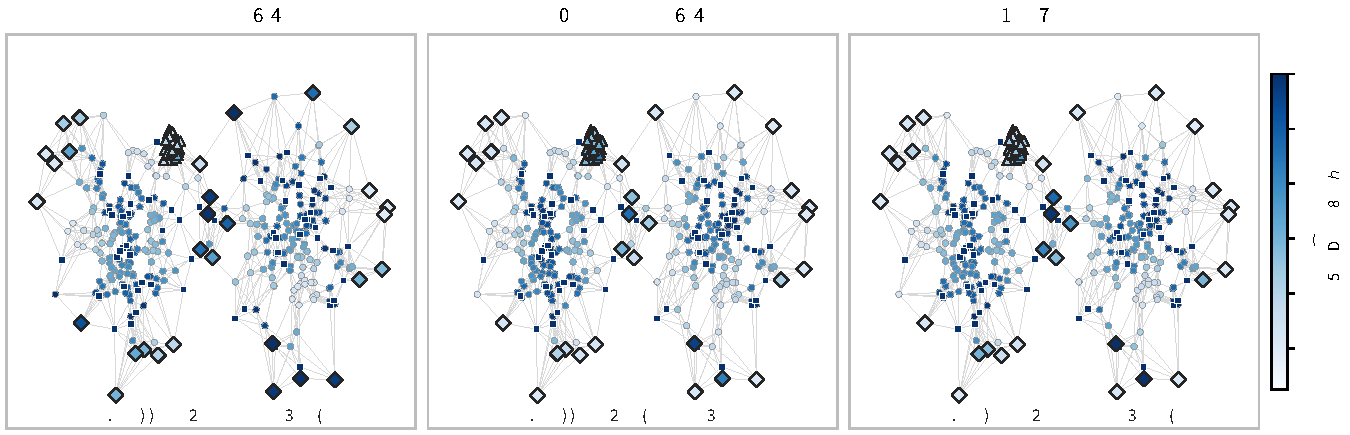
\includegraphics[width=\linewidth]{gen/fig_toy.pdf}
\caption{同じ量$h$と二つの代価（2次元の模式例；ガウス重みの対称な$k$近傍グラフ，$k{=}8$）．■は支持画像，○はIDのラベルなし画像，▲は密な未知の塊，◆は疎に散らばった未知で，色はラベルなし画像の中での$h$の順位（薄いほどOODらしい）．(a) 歩数の代価だけ（$\lambda{=}0.8$，$\gamma{=}0$）は塊を捉えるが散らばった未知を逃し，(b) 時間の代価だけ（$\lambda{=}1$，$\gamma$は次数の中央値の0.3倍）はその逆になり，(c) 二つの代価（$\lambda{=}0.8$，$\gamma$は0.03倍）は両方をIDより下に置く．種は使っていない．}
\label{fig:toy}
\end{figure}
v18の$u^{+}$は支持画像を吸収壁にしないので，$\lambda\to1$でランダムウォークが支持画像を通り抜けて定常分布に近づき，次数だけの量になる（(iii)）．$h$では支持画像に着いた時点で止まるので，極限\eqref{eq:cost}は到達までの費用という情報を持つ．ただし大きなランダム近傍グラフでは1点への到達時間が次数で決まる量に退化することが知られており~\cite{vonluxburg2014hitting}，$\lambda{=}1,\gamma{=}0$の調和関数もラベルなしの点が非常に多い極限で平坦になり得る~\cite{nadler2009limit}．本ノートが極限そのものではなく有限の代価$(\lambda,\gamma)$を使うのはこのためである．なお本ノートで使う$\lambda{=}0.95$は1次の領域から遠く（付録の(9)では$\varepsilon{=}10^{-2}$でも相対誤差\NCkLimTwo），期待費用は極限での読み方である．

\section{一つの読み出しと有効性}
\label{sec:valid}
\textbf{手続き．}(1) ラベル付き画像をクラスごとに支持画像12枚$\cS$，参照画像2枚$\cR$，較正画像2枚$\cC$に，画像に依らない位置で分ける．(2) 種なし（$\hQ=\emptyset$）の$h$を$h^{(0)}$とし，プール$\cU=\cC\cup\cT$の各画像の参照順位$p_{\cR}(u)=(1+|\{r\in\cR:h^{(0)}(r)\le h^{(0)}(u)\}|)/(|\cR|+1)$にStorey型のBH法（水準$q$，上限なしの$\hat\pi_0$，$\lambda_{\mathrm{S}}=\lfloor|\cR|/2\rfloor/(|\cR|+1)$）をかけて種$\hQ\subset\cU$を選ぶ．(3) 種を吸収壁にした$h$を解き，すべてのラベルなし画像を一歩先読みの値
\begin{equation}
s(x)=\rho_x\,(Ph)(x)=\frac{\lambda(Wh)(x)}{\delta_x+\gamma}
\label{eq:s}
\end{equation}
で採点する．種でない画像では$s=h$であり（命題1の証明），種では「そこから一歩跳んだ後に支持画像へ先に着く確率」（自分に戻れば種に着いたとみなす）である．(4) $p(x)=(1+|\{x'\in\cC:s(x')\le s(x)\}|)/(|\cC|+1)$とし（同点は独立な一様乱数で崩す．崩さずに$\le$で数えると定理2(i)は保守的になる），順位付けに$s$，判定に$p$を使う．較正集合が1つなので$p$は$s$の単調関数であり，同点を除いて同じ順序を与える．

\begin{theorem}[有効性]
$\cC$とIDのテスト画像が，他のすべての画像（$\cS$，$\cR$，未知のテスト画像）を所与として交換可能なら，
(i) IDのテスト画像$x$について$\Pr(p(x)\le\alpha)\le\alpha$，
(ii) $\{p(x)\}_{x\in\cT}$はIDの画像の上でPRDSで，水準$q$のBH法で選んだ集合の偽発見率は$q\,m_0/m$以下，Storey型（上限なしの$\hat\pi_0$，$\lambda_{\mathrm{S}}=\lfloor|\cC|/2\rfloor/(|\cC|+1)$）では$q$以下である（$m_0$はIDのテスト画像の数）．
(iii) さらに$\cR$とプールのIDの画像が交換可能なら，種の偽発見率も$q$以下である．
\end{theorem}
\begin{proof}
$s$は，ラベル付きの$\cS$，$\cR$と，$\cU$の画像の特徴の集まり（順序なし）だけの関数で，$\cU$の中でどの画像を較正画像と呼ぶかを入れ替えても各画像の値は変わらない．グラフは節点の名札に依らず，$h^{(0)}$は$\cS$を吸収壁とする同じ方程式の解，$p_{\cR}$は固定した$\cR$との比較，BH法はプールの$p_{\cR}$の多重集合から閾値を決めるので種の選び方は$\cU$の画像を対称に扱い，第2段の$h$と$s$も同様だからである．これはAdaDetect~\cite{marandon2024adadetect}の条件(8)で，$p$は同論文の経験$p$値(10)であり，同点を独立な一様乱数で崩せば同論文の同点なしの仮定も満たすので，定理3.3が(i)とPRDSを，系3.5と3.7が(ii)を与える．(iii)は$h^{(0)}$が$\cR\cup\cU$の中の置換に不変であることから，$\cR$を較正標本として同じ定理による．
\end{proof}

種を$\cT$だけから$\cC$に対する順位で選ぶと，$s$が「どの節点が較正画像か」に依存して条件(8)が崩れる．v18はこれを2つの折で回避したが，参照画像$\cR$を分けて較正画像も種の候補にすれば，折なしで条件が満たされる．代価はラベル付き画像の3分割で，較正画像はクラスあたり2枚（v18の折あたりと同じ）である．クラスごとに位置で固定した分割は$\cC$と$\cR$を層化するので，交換可能性は厳密には仮定である（v18の較正画像も同じ）．厳密にするには$\cC$と$\cR$をラベル付き画像から単純無作為に選べばよい．

\section{逃げる確率と捕まる確率}
\label{sec:sep}
両側の評価は一つの関数
\begin{equation}
\varphi(\rho,a,b)=\frac{\rho\,a}{1-\rho\,(1-a-b)}\qquad(0\le\rho\le1,\ a,b\ge0,\ a+b\le1;\ a=0\text{では}\varphi=0)
\label{eq:phi}
\end{equation}
で書ける．$\varphi$は$\rho$と$a$について増加，$b$について減少し，$\varphi\le1$，漏れがなければ$\varphi(1,a,b)=a/(a+b)$である．「出口$a$と出口$b$の競争に，1回の訪問ごとの生存率$\rho$が掛かる」と読める．

\begin{theorem}[逃げる確率：未知の側]
$Q\subset F$（支持画像も種も含まない）とし，$\partial Q$を$Q$に隣接する外の節点の集合とする．
(i) 出口分解：$Q$を初めて出る時刻を$\tau$，それまでのジャンプの回数を$N_\tau$とし，$H_Q(y,z)=\E_y[\lambda^{N_\tau}e^{-\gamma\tau};\ X_\tau=z]$として，$h(y)=\sum_{z\in\partial Q}H_Q(y,z)\,h(z)$（等式）．
(ii) 種でない外へ逃げる確率を$\pi_Q(y)=\sum_{z\in\partial Q\setminus\hQ}H_Q(y,z)$とすると，$h(y)\le\pi_Q(y)\max_{z\in\partial Q\setminus\hQ}h(z)\le\pi_Q(y)$．
(iii) $y\in Q$の重みのうち種でない外へ向かう割合を$e_y$，種へ向かう割合を$\zeta_y$とすると，$\pi_Q\le\varphi(\bar\rho,\bar e,\underline{\zeta})$（$\bar\rho=\max_Q\rho_y$，$\bar e=\max_Qe_y$，$\underline{\zeta}=\min_Q\zeta_y$）．
\end{theorem}

\begin{theorem}[捕まる確率：IDの側]
$B\subset F$とし，$y\in B$の重みのうち支持画像へ向かう割合を$\omega_y$，$B$にも$\cS$にも属さない節点へ向かう割合を$\eta_y$とする．$B$を出ずに支持画像に着く確率を$\kappa_B$とすると，$h\ge\kappa_B\ge\varphi(\underline{\rho},\underline{\omega},\bar\eta)$（$B$の上の最小・最大）．また，すべてのラベルなし画像で$s(x)\ge\rho_x\,\omega_x$である．
\end{theorem}

\begin{corollary}[分離]
種でないテスト画像$y$が定理3の$Q$に属し，各較正画像$x'$について$\ell(x')\le s(x')$（例えば定理4の$\rho_{x'}\omega_{x'}$．$x'$が種でなく$x'\in B$なら$\kappa_B(x')$でもよい）とすると，
\begin{equation}
p(y)\le\frac{1+|\{x'\in\cC:\ \ell(x')\le\pi_Q(y)\}|}{|\cC|+1}.
\label{eq:sep}
\end{equation}
特に$\pi_Q(y)<\min_{x'\in\cC}\ell(x')$なら$p(y)=1/(|\cC|+1)$であり，$y$は$\alpha\ge1/(|\cC|+1)$のすべての水準でOODと判定される．
\end{corollary}

\begin{proof}[定理3の証明]
(i) $Q$は支持画像も種も含まないので$\tau\le\tau_{\cS},\tau_{\hQ}$で，割引$\lambda^Ne^{-\gamma T}$は$\tau$の前後の積に分かれる（指数時間の無記憶性）．強マルコフ性から$h(y)=\E_y[\lambda^{N_\tau}e^{-\gamma\tau}h(X_\tau)]$．(ii) 種の上で$h=0$，$h\le1$から従う．(iii) $\pi=\pi_Q$は，$\mathcal{K}_Q(f)(y)=\rho_y\big(e_y+\sum_{j\in Q}P_{yj}f(j)\big)$の不動点のうち最小の非負解で，$0$から反復して得られる（滞在とジャンプを生き延び，種でない外へ出れば1，種へ出れば0，$Q$の中へ跳べばそこから続く）．$\sum_{j\in Q}P_{yj}=1-e_y-\zeta_y$だから定数$c\in[0,1]$に対し$\mathcal{K}_Q(c\mathbf{1})(y)=\rho_y(e_y+(1-e_y-\zeta_y)c)$で，これは$\rho_y,e_y$について増加，$\zeta_y$について減少する．$\bar\varphi=\varphi(\bar\rho,\bar e,\underline{\zeta})$は$\bar\varphi=\bar\rho(\bar e+(1-\bar e-\underline{\zeta})\bar\varphi)$を満たすので$\mathcal{K}_Q(\bar\varphi\mathbf{1})\le\bar\varphi\mathbf{1}$（優解）であり，$\mathcal{K}_Q$の単調性から反復の各段で$\mathcal{K}_Q^k(0)\le\bar\varphi\mathbf{1}$が保たれる．分母が0になるのは$\bar\rho=1$かつ$\bar e=\underline{\zeta}=0$のときだけで，$\bar e=0$なら$\pi\equiv0$（$\varphi=0$）である．
\end{proof}
\begin{proof}[定理4の証明]
$B$の中だけを通って支持画像に着く経路は種を通らないので$\kappa_B\le h$．$\kappa=\kappa_B$は$\mathcal{K}_B(f)(y)=\rho_y\big(\omega_y+\sum_{j\in B}P_{yj}f(j)\big)$の不動点で，$\sum_{j\in B}P_{yj}=1-\omega_y-\eta_y$．定理3と逆向きに，$\underline{\varphi}=\varphi(\underline{\rho},\underline{\omega},\bar\eta)$は$\mathcal{K}_B(\underline{\varphi}\mathbf{1})\ge\underline{\varphi}\mathbf{1}$（劣解）を満たし，$\mathcal{K}_B^k(\underline{\varphi}\mathbf{1})$は増加して不動点に収束する．$\bar\rho<1$なら$\mathcal{K}_B$は縮小写像で不動点は$\kappa$ただ一つ，$\lambda{=}1,\gamma{=}0$では$B$の各成分が出口を持てば一意で，出口のない成分があれば$\underline{\omega}=0$で$\underline{\varphi}=0$となり主張は自明である．最後の主張は$s(x)=\rho_x\sum_jP_{xj}h(j)\ge\rho_x\sum_{j\in\cS}P_{xj}$による（$h\ge0$，$\cS$の上で$h=1$）．
\end{proof}
\begin{proof}[系1の証明]
$y$は種でないので$s(y)=h(y)\le\pi_Q(y)$（定理3）．$s(x')\le s(y)$なら$\ell(x')\le s(x')\le\pi_Q(y)$．
\end{proof}

\textbf{読み方．}未知の塊$Q$では「種でない外への辺$e$」と「種への辺$\zeta$」が競い，IDの近傍では「支持画像への辺$\omega$」と「漏れる辺$\eta$」が競う．同じ$\varphi$が両側を抑え，その大小が較正順位の分離\eqref{eq:sep}を決める．種が効く理由はここにある：種を増やすと$h$は単調に減り（$\hQ\subset\hQ'$なら$\{\tau_{\cS}<\tau_{\hQ'}\}\subset\{\tau_{\cS}<\tau_{\hQ}\}$），塊のどの節点でも重みの割合$\underline{\zeta}$以上が種へ向かえば，漏れがなくても逃げる確率は$\bar e/(\bar e+\underline{\zeta})$以下になる．v18の系1の$\psi(e)=\lambda e/(1-\lambda+\lambda e)$は$\varphi(\lambda,e,0)$，すなわち$\gamma{=}0$・種なしの場合である．出口分解(i)は等式で，v18の命題2の係数$\lambda/(1-\lambda)$や$1/\min\sqrt{\delta}$は現れない．閉形式(iii)は最悪の節点で緩むが，$\pi_Q$は$Q$の上の小さな連立方程式で厳密に計算できる．

\section{クラスと粒度}
\begin{proposition}[クラスに依らない]
$\cS=\bigsqcup_c\cS_c$をIDのクラスへの分割とし，$h_c(x)$を最初に着く支持画像が$\cS_c$に属する確率（$\cS_c$で1，$(\cS\setminus\cS_c)\cup\hQ$で0の同じ方程式の解）とすると，$h=\sum_ch_c$．$h$はクラスの分け方に依らない．
\end{proposition}
\begin{proof}
事象$\{\tau_{\cS}<\tau_{\hQ}\}$は最初に着く支持画像のクラスで排反に分かれ，割引は共通である．
\end{proof}
同じグラフでクラスラベルを伝播させるLGC-maxは$\max_c$で読むので，近いIDクラスが複数ある画像では到達確率がそれらに割れて最大値が薄まる．$h$はその総和で，割れても変わらない．これはv18でクラスを捨てた構成がLGC-maxより良い理由の一つの説明であり，優越の定理ではない．

\begin{proposition}[粒度の床]
(i) $p\ge1/(|\cC|+1)$で，$p$は$1/(|\cC|+1)$刻みの値を取る．(ii) 種が選ばれるなら，その数は少なくとも$\hat\pi_0m/(q(|\cR|+1))$，すなわちプール$\cU$（大きさ$m$）の割合$\hat\pi_0/(q(|\cR|+1))$以上である．
\end{proposition}
\begin{proof}
(ii) BH法の棄却数$\hat k\ge1$は$p_{(\hat k)}\le q\hat k/(\hat\pi_0m)$を満たし，$p_{(\hat k)}\ge1/(|\cR|+1)$だから$\hat k\ge\hat\pi_0m/(q(|\cR|+1))$．
\end{proof}
この下限はdev1（$|\cR|=1{,}800$，$q{=}0.2$）ではプールの約\NFloorFrac\%（$\hat\pi_0$倍），ImageNet-1Kのテスト集合（$|\cR|=2{,}000$）では約0.25\%で，v18の折の閾値と同じである．これは共形$p$値の分解能$1/(n+1)$そのものから来る構造である．

\section{dev1での探索（登録外）}
\label{sec:dev1}
以下は開発用分割dev1だけで行った探索である（dev2とテスト集合には触れていない）．dev1はImageNet-1Kの学習画像だけから作った分割で，900クラスをID（支持画像\NNs{}枚，較正画像\NNc{}枚，IDのテスト画像\NNid{}枚）とし，未知のnear \NNoodNear{}枚，far \NNoodFar{}枚を加える（5通りの抽出の平均，単体，DINOv2 L/14 + DINOv3 L/16，$k_g{=}10$，種はStorey型$q{=}0.2$）．試した構成は参照を除いて\NNCfg{}通りで，最後の構成はこれらの値を見て決めたため，dev1の値は楽観的である．

\begin{table}[t]
\centering
\caption{dev1での読み出しの比較（[\%]，単体，5通りの抽出の平均）．誤警報率はIDのテスト画像のうち$p\le0.05$となった割合（共形$p$値を返す構成のみ）．太字は列の最良．}
\label{tab:main}
\small
\setlength{\tabcolsep}{4pt}
\begin{tabular}{lcccccc}
\toprule
 & \multicolumn{2}{c}{dev1 far} & \multicolumn{2}{c}{dev1 near} & \multicolumn{2}{c}{誤警報率（$\alpha{=}0.05$）}\\
\cmidrule(lr){2-3}\cmidrule(lr){4-5}\cmidrule(lr){6-7}
構成 & \AUC$\uparrow$ & \FPR$\downarrow$ & \AUC$\uparrow$ & \FPR$\downarrow$ & far & near\\
\midrule
\multicolumn{7}{l}{\textit{v18の読み出し（参照）}}\\
\quad $\sigma$（$\pP\pN$，2折） & 96.69 & 16.74 & \textbf{97.09} & 13.69 & 0.051 & 0.050\\
\quad $\pP$のみ & 96.51 & 16.30 & 95.67 & 18.75 & -- & --\\
\midrule
\multicolumn{7}{l}{\textit{歩数の代価だけ（$\gamma{=}0$）}}\\
\quad 種なし，$\lambda{=}0.9$ & 90.74 & 28.27 & 96.02 & \textbf{13.43} & 0.047 & 0.052\\
\quad 種（2折），$\lambda{=}0.9$ & 92.01 & 24.40 & 96.63 & 13.81 & 0.049 & 0.051\\
\quad 種（折なし），$\lambda{=}0.9$ & 91.65 & 25.35 & 96.53 & 14.19 & 0.049 & 0.051\\
\quad 種（折なし），$\lambda{\to}1$：調和関数 & 93.57 & 26.15 & 96.83 & 14.38 & 0.050 & 0.050\\
\quad 種なし，$\lambda{\to}1$：$-\mathbb{E}[N_{\mathcal{S}}]$ & 91.31 & 27.16 & 96.27 & 14.26 & 0.048 & 0.052\\
\quad 有向$k_g$近傍，種なし & 87.87 & 38.92 & 95.20 & 16.36 & 0.047 & 0.050\\
\midrule
\multicolumn{7}{l}{\textit{時間の代価だけ（$\lambda{=}1$）}}\\
\quad 種なし，$\gamma{=}1$ & 96.70 & 15.53 & 95.67 & 19.27 & 0.049 & 0.051\\
\quad 種（2折），$\gamma{=}1$ & \textbf{96.77} & 15.84 & 96.29 & 16.34 & 0.050 & 0.049\\
\quad 種なし，$\gamma{\to}0$：$-\mathbb{E}[T_{\mathcal{S}}]$ & 96.72 & \textbf{15.29} & 95.71 & 19.81 & 0.049 & 0.052\\
\midrule
\multicolumn{7}{l}{\textit{二つの代価（$\lambda{=}0.95$，$\gamma\approx\mathrm{median}(\delta)/16$）}}\\
\quad 種なし & 96.10 & 17.74 & 96.28 & 15.38 & 0.048 & 0.052\\
\quad 種（2折），和グラフ & 96.27 & 16.79 & 96.71 & 14.16 & 0.048 & 0.050\\
\quad 種（2折），ビューごと＋順位の積 & 96.21 & 16.69 & 96.69 & 13.51 & 0.047 & 0.050\\
\quad 折なし，$\mathcal{S}$11/$\mathcal{R}$1/$\mathcal{C}$4 & 96.05 & 17.55 & 96.64 & 14.46 & 0.049 & 0.049\\
\quad 折なし，12/2/2，ビューごと & 96.27 & 16.74 & 96.73 & 13.72 & 0.048 & 0.051\\
\quad \textbf{折なし，12/2/2，正規化和：一つの量} & 96.34 & 16.77 & 96.80 & 13.74 & 0.049 & 0.050\\
\bottomrule
\end{tabular}

\end{table}

\textbf{支持画像と種を吸収壁にするだけでは，farで負ける．}歩数の代価だけのランダムウォーク（$\gamma{=}0$）は，種なしでもnearで\NAbsOneNear\%と$\sigma$（\NSigNear\%）に並ぶが，farは\NAbsOneFar\%と$\sigma$（\NSigFar\%）より\NAbsOneGapFar{}ポイント悪い（\tabref{tab:main}）．種を加えても（\NAbsXfitFar\%），$\lambda\to1$の調和関数でも（\NHarmFar\%），有向の近傍でも（\NDirFar\%）farの劣勢は残る．

\begin{table}[t]
\centering
\caption{v18の$u^{+}$の次数成分（dev1，5通りの抽出の平均）．\AUC$(\delta)$，\FPR$(\delta)$は次数$\delta$だけをスコアにした値．}
\label{tab:deg}
\small
\begin{tabular}{llccccc}
\toprule
未知 & ビュー & Spearman$(u^{+},\sqrt{\delta})$ & \AUC$(\delta)$ & \FPR$(\delta)$ & \FPR$(u^{+})$ & \FPR$(u^{+}/\sqrt{\delta})$\\
\midrule
far & DINOv2 L/14 & 0.80 & 86.7 & 61.6 & 21.8 & 54.3\\
far & DINOv3 L/16 & 0.82 & 82.2 & 70.6 & 18.9 & 41.7\\
near & DINOv2 L/14 & 0.46 & 49.1 & 95.5 & 22.9 & 19.9\\
near & DINOv3 L/16 & 0.50 & 48.6 & 95.8 & 22.2 & 15.9\\
\bottomrule
\end{tabular}

\end{table}

\textbf{原因は$\sqrt{\delta}$が運んでいた密度である．}v18の$u^{+}$はfarでは$\sqrt{\delta}$と強く相関し（Spearman \NDegSpFarL{}，\NDegSpFarD），次数だけで\AUC{}が\NDegAucFarL{}／\NDegAucFarD\%に達する（\tabref{tab:deg}）．$u^{+}$を$\sqrt{\delta}$で割って確率の部分だけにすると，farの\FPR{}は\NUFprFarL{}から\NUnFprFarL\%（DINOv2），\NUFprFarD{}から\NUnFprFarD\%（DINOv3）へ崩れ，nearでは逆に\NUFprNearL{}から\NUnFprNearL\%，\NUFprNearD{}から\NUnFprNearD\%へ良くなる．v18で「順位付けは$u$，確率の意味は$u/\sqrt{\delta}$」とずれていた$\sqrt{\delta}$は，farの手がかりそのものであった．時間の代価だけの量（$\lambda{=}1$）はその逆で，到達時間$-\E[T_{\cS}]$はfarで\NCtHitFar\%と表の最良に近く，nearは\NCtHitNear\%と悪い．

\begin{table}[t]
\centering
\caption{$\lambda\times\gamma$の格子（dev1の\FPR{} [\%]，far\,/\,near；和グラフ$W_{\mathrm{L14}}+W_{\mathrm{D3L}}$の上の1本のランダムウォーク）．$\gamma{=}1$は和グラフの次数の中央値（\NMedDegLo--\NMedDegHi）の約1/16．}
\label{tab:grid}
\small
\begin{tabular}{lccc|ccc}
\toprule
 & \multicolumn{3}{c|}{種なし（$\mathcal{S}$だけが吸収壁）} & \multicolumn{3}{c}{種（2折）}\\
$\lambda$ \textbackslash{} $\gamma$ & 0.3 & 1 & 3 & 0.3 & 1 & 3\\
\midrule
0.8 & 26.5\,/\,14.3 & 22.6\,/\,14.7 & 19.4\,/\,16.8 & 24.0\,/\,13.9 & 21.3\,/\,14.2 & 18.7\,/\,15.3\\
0.9 & 23.6\,/\,13.6 & 19.6\,/\,14.6 & 17.6\,/\,17.5 & 21.3\,/\,13.7 & 18.4\,/\,13.9 & 16.9\,/\,15.5\\
0.95 & 20.9\,/\,13.7 & 17.7\,/\,15.4 & 16.8\,/\,18.3 & 19.5\,/\,13.5 & 16.8\,/\,14.2 & 16.3\,/\,15.8\\
\midrule
\multicolumn{7}{l}{参照：$\sigma$ 16.7\,/\,13.7，$\pP$のみ 16.3\,/\,18.7，$\gamma{=}0$・$\lambda{=}0.9$の種なし 28.3\,/\,13.4}\\
\bottomrule
\end{tabular}

\end{table}

\textbf{二つの代価で両方が戻る．}$\gamma$を大きくするとfarが良くnearが悪くなり，$\lambda$を0.8から0.95へ上げるとfarはどの$\gamma$でも良くなる（nearは$\gamma$が小さいとき並び，$\gamma{=}1$では$\lambda{=}0.9$がわずかに良い；\tabref{tab:grid}）．$\lambda{=}0.95$，$\gamma$を次数の中央値の1/16とした上で，折をなくし，ラベル付き画像をクラスごとに12/2/2に分け，ビューの重みをそれぞれの次数の中央値で割って足した1つのグラフで一つの量$h$を解く構成（\tabref{tab:main}の最下行）は，farで\NFinFar\%，nearで\NFinNear\%と$\sigma$に並ぶ．抽出を単位とする対応のある差（一つの量$-\sigma$）の95\%区間はfar [\NFinDiffFarLo, \NFinDiffFarHi]，near [\NFinDiffNearLo, \NFinDiffNearHi]ポイントである．\AUC{}は\NFinFarAuc{}／\NFinNearAuc\%で，$\sigma$より\NFinAucGapFar{}／\NFinAucGapNear{}ポイント低い．IDの誤警報率は$\alpha{=}0.05$で\NFinFarVal{}／\NFinNearVal{}，$\alpha{=}0.2$で\NFinFarValTwo{}／\NFinNearValTwo{}と水準どおりで，種は平均\NFinFarSeeds{}／\NFinNearSeeds{}枚（IDの割合\NFinFarIdf{}／\NFinNearIdf\%，うち較正画像\NFinFarCalSeeds{}／\NFinNearCalSeeds{}枚）である．参照画像をクラスあたり1枚にすると（支持画像11枚，較正画像4枚）\NPoolOneFar{}／\NPoolOneNear\%と悪く，ビューを和でなく順位の積で合わせても\NPoolPFar{}／\NPoolPNear\%と変わらない．

\section{20の継ぎ目}
\label{sec:seams}
\begin{table}[t]
\centering
\caption{20の継ぎ目と，一つの量$h$での状態．解消13，説明3，一部3，残る1．}
\label{tab:seams}
\footnotesize
\setlength{\tabcolsep}{3pt}
\renewcommand{\arraystretch}{1.12}
\begin{tabular}{rp{0.33\linewidth}cp{0.52\linewidth}}
\toprule
& 継ぎ目 & 状態 & 一つの量$h$で \\
\midrule
1 & 有効性と検知力が別の理論 & 解消 & 同じ$s$について定理2（有効性）と定理3・4が述べ，系1で一つになる．\\
2 & 未知側の上界だけで分離定理でない & 解消 & 定理4（IDの下界）と系1（分離）．\\
3 & v18の命題1が使われず，記述も不正確 & 解消 & $h$は確率で尺度が絶対的（$[0,1]$）．質量の保存は要らず，v18の命題1は削る．\\
4 & 種が効く理由に定理がない & 解消 & 定理3：種への出口は逃げる確率から除かれ，種を増やすと$h$は単調に減る．各節点が種に接すれば漏れなしでも$\pi_Q\le\bar e/(\bar e+\underline{\zeta})$．\\
5 & v18の命題2の係数が緩く，系1も情報を捨てる & 解消 & 出口分解は等式．$\lambda/(1-\lambda)$も$1/\min\sqrt{\delta}$も現れず，$\pi_Q$は厳密に解ける．\\
6 & クラスを捨てる方が良い理由がない & 説明 & 本ノートの命題3：$h=\sum_ch_c$．最大値は近いクラスの間で割れる（優越の定理ではない）．\\
7 & 積$\pP\pN$に確率の意味がない & 解消 & 一つの確率$h$．本ノートの命題2で三つの行き先が排反になる．\\
8 & 出力が2つ（$\sigma$と$\pfin$）& 解消 & 較正集合が1つなので$p$は$s$の単調関数で，同点を除き同じ順序を与える．\\
9 & 順位の順位 & 解消 & 最終の読み出しは確率$s$の順位で，順位の関数をまた順位で読むことはない（参照順位は種の選択にだけ使う）．\\
10 & $s_0\exp\sigma$は保証の外 & 残る & ベース検出器は較正画像のスコアを持たない．較正画像をベース検出器の入力に無作為に混ぜる形は未検討．\\
11 & 変種が4つ & 一部 & 種の規則（BH／Storey$\times$上限）は零境界$\hQ$の選び方の違いになる．定理2(i)(ii)と定理3・4は$\cU$を対称に扱うどの規則でも成り立つ（種の偽発見率(iii)はBH／Storey型について）．選択は残る．\\
12 & 順位は$u$，確率は$u/\sqrt{\delta}$ & 解消 & $h$そのものが確率．$\sqrt{\delta}$が運んでいた密度は時間の代価$\gamma$として意味を持って戻る．\\
13 & 支持画像が吸収壁でなく，$\lambda\to1$で次数だけ & 解消 & 支持画像は吸収壁．$\lambda\to1$の極限は到達までの費用（定理1）で，$u^{+}$のように恒等的に次数だけにはならない（大きなグラフでの退化の可能性は\S\ref{sec:prices}の注意）．\\
14 & $W=\max(A,A^{\top})$が外からの辺を生む & 説明 & 対称性がディリクレ原理（エネルギー・回路）を与える．有向の近傍では互いの近傍に閉じた$r\ge k_g+1$枚の塊から出られず$h=0$になるが，dev1のfarで\NDirFar\%と悪い．\\
15 & 支持画像と種が対称でない & 解消 & 両者は同じ方程式の境界（1と0）で，$\lambda{=}1,\gamma{=}0$なら入れ替えで$h\mapsto1-h$．種は較正画像を含むプールから選ぶ．\\
16 & $1/(n'+1)$の床，0.25\%の閾値 & 説明 & 本ノートの命題4：共形$p$値の分解能そのもの．種が選ばれるならその数はプールの$\hat\pi_0/(q(|\cR|+1))$以上．\\
17 & 交差適合が1回の分割に依存，FDRは折ごと & 解消 & 乱数の折がない．偽発見率はテスト集合全体で保証される（$\cS/\cR/\cC$の分け方は位置で固定）．\\
18 & 定数に導出がない & 一部 & 2折は消え，$\lambda,\gamma$は歩数と時間の代価という意味と極限を持ち，$\gamma$は次数の中央値で無次元化される．$k_g$，$q$，12/2/2は選ぶ量として残る．\\
19 & ビューの統合が順位の積 & 解消 & 正規化した重みの和の1つのグラフ上の1本のランダムウォーク．\\
20 & 証明する量と報告する量が違う & 一部 & 系1は「水準$\alpha$で検知される」形で保証と順位をつなぐが，\AUC{}・\FPR{}の定理ではない．交換可能な較正を要する点も変わらない．\\
\bottomrule
\end{tabular}
\end{table}
\tabref{tab:seams}に，20の継ぎ目それぞれの状態をまとめる．1〜5は定理2〜4と系1で一つにつながり，7・12・13は同じ根（支持画像と種を吸収壁にしない2本の質量）から出ていたものが一度に消える．ただし12は「$\sqrt{\delta}$を消す」のではなく「$\sqrt{\delta}$が運んでいた密度を時間の代価として確率の中に置き直す」ことで解消する．これを怠ると\S\ref{sec:dev1}のとおりfarを失う．

\section{次の段：Phase 16の登録案}
(1) \textbf{登録}：構成を一つに固定する（$\lambda{=}0.95$，$\gamma$は次数の中央値の1/16，正規化した和グラフ，12/2/2，Storey型$q{=}0.2$，折なし，一歩先読み）．ベース検出器との合わせ方（例えば$s_0\cdot h$；定理2の外で，順位付けのためだけ）もdev1で決めて同時に登録する．dev2での仮説はH1：nearの\FPR{}の差（一つの量$-\sigma$，5通りの抽出の平均の点推定）$\le+0.5$，H2：farで同じ，H3：単体の$p$の$\alpha\in\{0.05,0.2\}$での誤警報率が水準どおり．区間も併記する．H1かつH2なら主構成をこの量に替える．どの結果も報告する．(2) \textbf{テスト集合}（凍結）：OpenOOD v1.5 ImageNet-1Kのnear/far，Four-OOD（6通りの抽出，4つのベース検出器），ImageNet-200，CIFAR-100，再出現の枚数$\times$混入率の格子．(3) \textbf{記述的な確認}（登録外）：定理3・4と系1の評価がどこまで締まるかを，再出現の格子で測る．(4) \textbf{論文}：採用なら提案手法を「一つの問い」から書き直し（定義，三つの表示，二つの代価，定理2〜4，系1），v18の$\sigma$は比較の行にする．不採用なら本ノートの\S1--6を付録に置く．

\begin{thebibliography}{99}
\setlength{\itemsep}{0pt}
\footnotesize
\bibitem{zhu2003harmonic} X.~Zhu, Z.~Ghahramani, J.~Lafferty. Semi-supervised learning using Gaussian fields and harmonic functions. ICML, 2003.
\bibitem{grady2006rw} L.~Grady. Random walks for image segmentation. IEEE TPAMI, 28(11):1768--1783, 2006.
\bibitem{wu2012parw} X.-M.~Wu, Z.~Li, A.~M.-C.~So, J.~Wright, S.-F.~Chang. Learning with partially absorbing random walks. NeurIPS, 2012.
\bibitem{doyle1984} P.~G.~Doyle, J.~L.~Snell. Random Walks and Electric Networks. Mathematical Association of America, 1984.
\bibitem{vonluxburg2014hitting} U.~von Luxburg, A.~Radl, M.~Hein. Hitting and commute times in large random neighborhood graphs. JMLR, 15:1751--1798, 2014.
\bibitem{nadler2009limit} B.~Nadler, N.~Srebro, X.~Zhou. Statistical analysis of semi-supervised learning: The limit of infinite unlabelled data. NeurIPS, 2009.
\bibitem{marandon2024adadetect} A.~Marandon, L.~Lei, D.~Mary, E.~Roquain. Adaptive novelty detection with false discovery rate guarantee. Annals of Statistics, 52(1):157--183, 2024.
\bibitem{zhou2004lgc} D.~Zhou, O.~Bousquet, T.~N.~Lal, J.~Weston, B.~Sch\"{o}lkopf. Learning with local and global consistency. NeurIPS, 2004.
\end{thebibliography}
\clearpage
\appendix
\section{合成データでの数値確認}
各主張を合成データで確かめた（\texttt{theory16\_checks.py}；64次元，IDの100クラス，支持画像12枚・参照画像2枚，IDの画像2,400枚を較正画像400枚とテスト画像に無作為に分け，20枚ずつの密な未知10クラスと散らばった未知200枚，$k_g{=}10$，$\lambda{=}0.95$，$\gamma$は次数の中央値の1/16）．(11)は合成データを\NCkReps{}回作り直した平均である．等式の主張（(2)〜(6)）は数値誤差の範囲で成り立ち，不等式の主張（(6)〜(8)）に違反はない．(8)では上界だけで種でない未知の\NCkSepELeBnd\%に$p\le0.05$が保証される（逃げる確率の中央値\NCkSepEPi，較正画像の$\rho\omega$の中央値\NCkSepERhoOm）．(11)の偽発見割合は$q\,m_0/m=\NCkQmm$以下に収まる．対照として種を$\cT$だけから$\cC$との比較で選ぶと，$\alpha{=}0.05$での誤警報率は\NCkTonlyFive{}（標準誤差\NCkTonlyFiveSe）と水準を超え，定理2の置換不変性が飾りでないことを示す．
\begin{center}
\small
\begin{tabular}{p{0.30\linewidth}p{0.42\linewidth}p{0.20\linewidth}}
\toprule
主張 & 測った量 & 結果\\
\midrule
(1) 線形方程式 $=$ ランダムウォーク & 解とモンテカルロ（2万回）の差の最大（標準誤差の倍数） & 0.9\\
(2) エネルギー最小・キルヒホッフ則 & 自由節点の電流の収支の最大残差；摂動200回がすべて増加 & 2e-14；はい\\
(3) 尺度の共変性 $h(cW;\lambda,c\gamma)=h(W;\lambda,\gamma)$ & 最大差 & 2e-15\\
(4) 三つの行き先の確率の和 $=1$ & 1からのずれの最大 & 2e-15\\
(5) クラスごとの到達確率の和 $=h$ & 最大差 & 2e-15\\
(6) 出口分解（等式），$h\le\pi_Q\le\varphi$ & 分解の誤差の最大；10の塊で$h\le\pi_Q$，$\pi_Q\le\varphi$ & 6e-17；すべて成立\\
(7) 捕まる確率の下界 & 8クラスで$h\ge\kappa\ge\varphi$，$\kappa\ge\rho\omega$ & すべて成立\\
(8) 分離（系1）& 密な未知の塊（種は各塊の5枚に1枚）の種でない160枚：違反数，上界だけで$p\le0.05$が保証される割合（実際）；全手続きの種でない未知154枚での違反数 & 0，94\%（100\%）；0\\
(9) 1次の極限 $(1-h)/\varepsilon\to\mu\mathbb{E}N+\nu\mathbb{E}T$ & 相対誤差の最大（$\varepsilon{=}10^{-2}$，$10^{-4}$）& 0.77，0.031\\
(10) LGCの$u^{+}\to\sqrt{\delta}$（$\lambda\to1$）& Spearman$(u^{+},\sqrt\delta)$（$\lambda{=}0.9\to0.9999$）& 0.55$\to$0.9998\\
(11) 有効性（定理2），400回 & $\alpha{=}0.05/0.1/0.2$でのIDの誤警報率；BH($q{=}0.2$)の偽発見割合 & 0.050/0.101/0.201；0.155\\
\quad 対照：種を$\mathcal{C}$で認定（置換不変でない）& 同上 & 0.054/0.104/0.202；0.175\\
\bottomrule
\end{tabular}

\end{center}

\end{document}
